\section{eo\-Timed\-State\-Saver Class Reference}
\label{classeo_timed_state_saver}\index{eoTimedStateSaver@{eoTimedStateSaver}}
an {\bf eo\-Updater}{\rm (p.\,\pageref{classeo_updater})} that saves a state every given time interval  


{\tt \#include $<$eo\-Updater.h$>$}

Inheritance diagram for eo\-Timed\-State\-Saver::\begin{figure}[H]
\begin{center}
\leavevmode
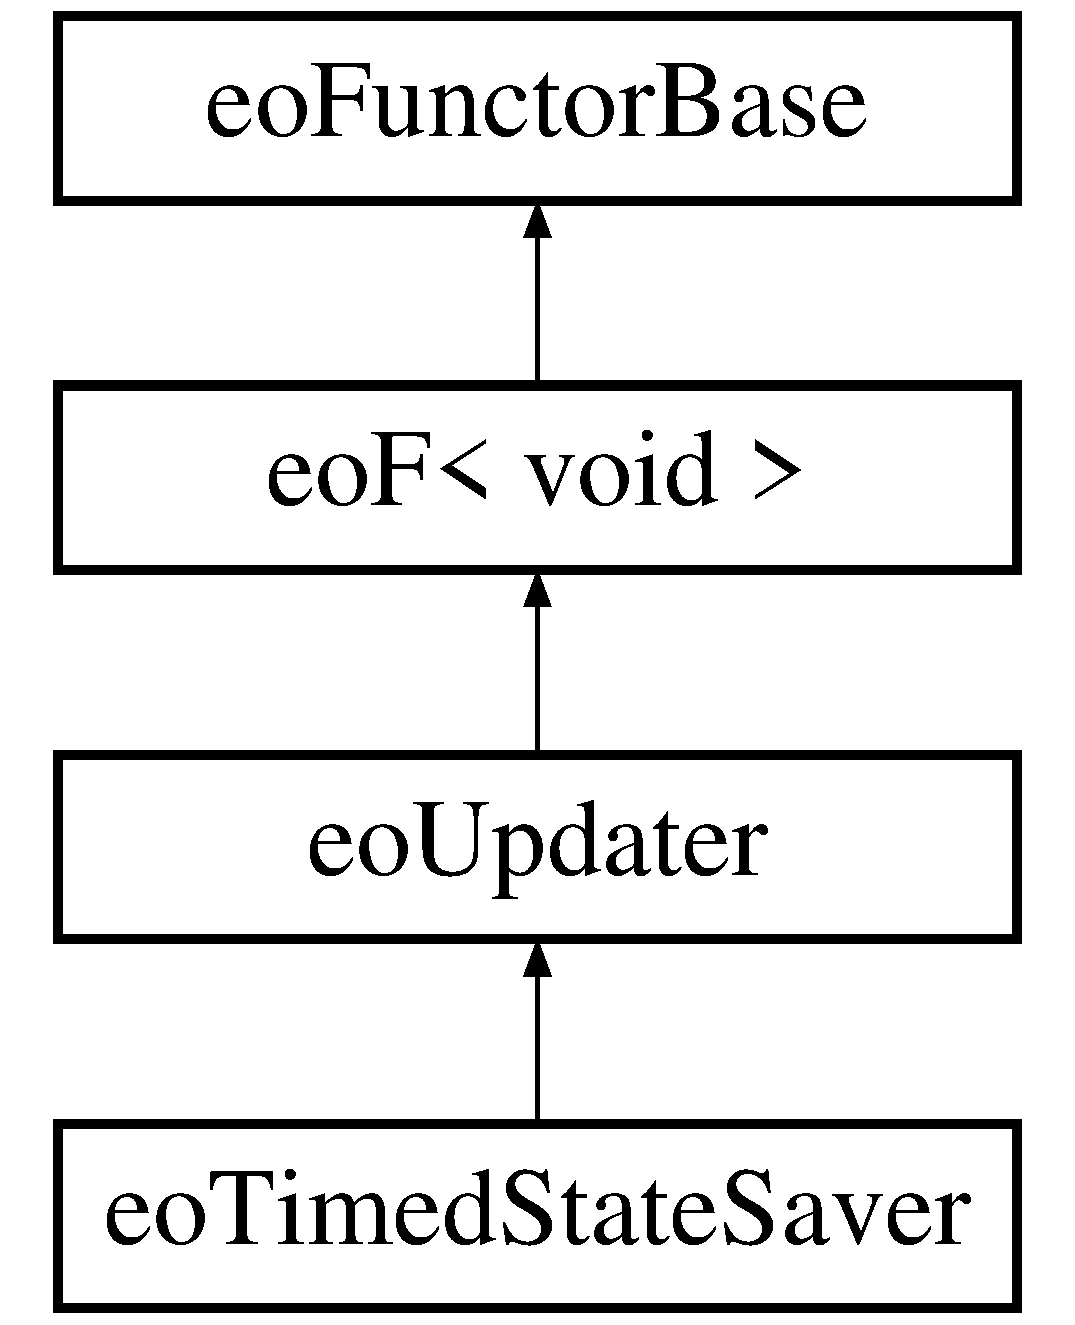
\includegraphics[height=4cm]{classeo_timed_state_saver}
\end{center}
\end{figure}
\subsection*{Public Member Functions}
\begin{CompactItemize}
\item 
{\bf eo\-Timed\-State\-Saver} (time\_\-t \_\-interval, const {\bf eo\-State} \&\_\-state, std::string \_\-prefix=\char`\"{}state\char`\"{}, std::string \_\-extension=\char`\"{}sav\char`\"{})\label{classeo_timed_state_saver_a0}

\item 
void {\bf operator()} (void)\label{classeo_timed_state_saver_a1}

\begin{CompactList}\small\item\em The pure virtual function that needs to be implemented by the subclass. \item\end{CompactList}\item 
virtual std::string {\bf class\-Name} (void) const \label{classeo_timed_state_saver_a2}

\end{CompactItemize}
\subsection*{Private Attributes}
\begin{CompactItemize}
\item 
const {\bf eo\-State} \& {\bf state}\label{classeo_timed_state_saver_r0}

\item 
const time\_\-t {\bf interval}\label{classeo_timed_state_saver_r1}

\item 
time\_\-t {\bf last\_\-time}\label{classeo_timed_state_saver_r2}

\item 
const time\_\-t {\bf first\_\-time}\label{classeo_timed_state_saver_r3}

\item 
const std::string {\bf prefix}\label{classeo_timed_state_saver_r4}

\item 
const std::string {\bf extension}\label{classeo_timed_state_saver_r5}

\end{CompactItemize}


\subsection{Detailed Description}
an {\bf eo\-Updater}{\rm (p.\,\pageref{classeo_updater})} that saves a state every given time interval 



Definition at line 104 of file eo\-Updater.h.

The documentation for this class was generated from the following files:\begin{CompactItemize}
\item 
eo\-Updater.h\item 
eo\-Updater.cpp\end{CompactItemize}
